\documentclass[1p]{elsarticle_modified}
%\bibliographystyle{elsarticle-num}

%\usepackage[colorlinks]{hyperref}
%\usepackage{abbrmath_seonhwa} %\Abb, \Ascr, \Acal ,\Abf, \Afrak
\usepackage{amsfonts}
\usepackage{amssymb}
\usepackage{amsmath}
\usepackage{amsthm}
\usepackage{scalefnt}
\usepackage{amsbsy}
\usepackage{kotex}
\usepackage{caption}
\usepackage{subfig}
\usepackage{color}
\usepackage{graphicx}
\usepackage{xcolor} %% white, black, red, green, blue, cyan, magenta, yellow
\usepackage{float}
\usepackage{setspace}
\usepackage{hyperref}

\usepackage{tikz}
\usetikzlibrary{arrows}

\usepackage{multirow}
\usepackage{array} % fixed length table
\usepackage{hhline}

%%%%%%%%%%%%%%%%%%%%%
\makeatletter
\renewcommand*\env@matrix[1][\arraystretch]{%
	\edef\arraystretch{#1}%
	\hskip -\arraycolsep
	\let\@ifnextchar\new@ifnextchar
	\array{*\c@MaxMatrixCols c}}
\makeatother %https://tex.stackexchange.com/questions/14071/how-can-i-increase-the-line-spacing-in-a-matrix
%%%%%%%%%%%%%%%

\usepackage[normalem]{ulem}

\newcommand{\msout}[1]{\ifmmode\text{\sout{\ensuremath{#1}}}\else\sout{#1}\fi}
%SOURCE: \msout is \stkout macro in https://tex.stackexchange.com/questions/20609/strikeout-in-math-mode

\newcommand{\cancel}[1]{
	\ifmmode
	{\color{red}\msout{#1}}
	\else
	{\color{red}\sout{#1}}
	\fi
}

\newcommand{\add}[1]{
	{\color{blue}\uwave{#1}}
}

\newcommand{\replace}[2]{
	\ifmmode
	{\color{red}\msout{#1}}{\color{blue}\uwave{#2}}
	\else
	{\color{red}\sout{#1}}{\color{blue}\uwave{#2}}
	\fi
}

\newcommand{\Sol}{\mathcal{S}} %segment
\newcommand{\D}{D} %diagram
\newcommand{\A}{\mathcal{A}} %arc


%%%%%%%%%%%%%%%%%%%%%%%%%%%%%5 test

\def\sl{\operatorname{\textup{SL}}(2,\Cbb)}
\def\psl{\operatorname{\textup{PSL}}(2,\Cbb)}
\def\quan{\mkern 1mu \triangleright \mkern 1mu}

\theoremstyle{definition}
\newtheorem{thm}{Theorem}[section]
\newtheorem{prop}[thm]{Proposition}
\newtheorem{lem}[thm]{Lemma}
\newtheorem{ques}[thm]{Question}
\newtheorem{cor}[thm]{Corollary}
\newtheorem{defn}[thm]{Definition}
\newtheorem{exam}[thm]{Example}
\newtheorem{rmk}[thm]{Remark}
\newtheorem{alg}[thm]{Algorithm}

\newcommand{\I}{\sqrt{-1}}
\begin{document}

%\begin{frontmatter}
%
%\title{Boundary parabolic representations of knots up to 8 crossings}
%
%%% Group authors per affiliation:
%\author{Yunhi Cho} 
%\address{Department of Mathematics, University of Seoul, Seoul, Korea}
%\ead{yhcho@uos.ac.kr}
%
%
%\author{Seonhwa Kim} %\fnref{s_kim}}
%\address{Center for Geometry and Physics, Institute for Basic Science, Pohang, 37673, Korea}
%\ead{ryeona17@ibs.re.kr}
%
%\author{Hyuk Kim}
%\address{Department of Mathematical Sciences, Seoul National University, Seoul 08826, Korea}
%\ead{hyukkim@snu.ac.kr}
%
%\author{Seokbeom Yoon}
%\address{Department of Mathematical Sciences, Seoul National University, Seoul, 08826,  Korea}
%\ead{sbyoon15@snu.ac.kr}
%
%\begin{abstract}
%We find all boundary parabolic representation of knots up to 8 crossings.
%
%\end{abstract}
%\begin{keyword}
%    \MSC[2010] 57M25 
%\end{keyword}
%
%\end{frontmatter}

%\linenumbers
%\tableofcontents
%
\newcommand\colored[1]{\textcolor{white}{\rule[-0.35ex]{0.8em}{1.4ex}}\kern-0.8em\color{red} #1}%
%\newcommand\colored[1]{\textcolor{white}{ #1}\kern-2.17ex	\textcolor{white}{ #1}\kern-1.81ex	\textcolor{white}{ #1}\kern-2.15ex\color{red}#1	}

{\Large $\underline{12n_{0657}~(K12n_{0657})}$}

\setlength{\tabcolsep}{10pt}
\renewcommand{\arraystretch}{1.6}
\vspace{1cm}\begin{tabular}{m{100pt}>{\centering\arraybackslash}m{274pt}}
\multirow{5}{120pt}{
	\centering
	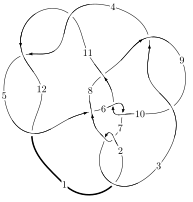
\includegraphics[width=112pt]{../../../GIT/diagram.site/Diagrams/png/2746_12n_0657.png}\\
\ \ \ A knot diagram\footnotemark}&
\allowdisplaybreaks
\textbf{Linearized knot diagam} \\
\cline{2-2}
 &
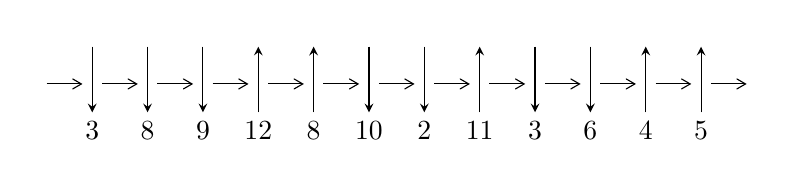
\begin{tikzpicture}[x=20pt, y=17pt]
	% nodes
	\node (C0) at (0, 0) {};
	\node (C1) at (1, 0) {};
	\node (C1U) at (1, +1) {};
	\node (C1D) at (1, -1) {3};

	\node (C2) at (2, 0) {};
	\node (C2U) at (2, +1) {};
	\node (C2D) at (2, -1) {8};

	\node (C3) at (3, 0) {};
	\node (C3U) at (3, +1) {};
	\node (C3D) at (3, -1) {9};

	\node (C4) at (4, 0) {};
	\node (C4U) at (4, +1) {};
	\node (C4D) at (4, -1) {12};

	\node (C5) at (5, 0) {};
	\node (C5U) at (5, +1) {};
	\node (C5D) at (5, -1) {8};

	\node (C6) at (6, 0) {};
	\node (C6U) at (6, +1) {};
	\node (C6D) at (6, -1) {10};

	\node (C7) at (7, 0) {};
	\node (C7U) at (7, +1) {};
	\node (C7D) at (7, -1) {2};

	\node (C8) at (8, 0) {};
	\node (C8U) at (8, +1) {};
	\node (C8D) at (8, -1) {11};

	\node (C9) at (9, 0) {};
	\node (C9U) at (9, +1) {};
	\node (C9D) at (9, -1) {3};

	\node (C10) at (10, 0) {};
	\node (C10U) at (10, +1) {};
	\node (C10D) at (10, -1) {6};

	\node (C11) at (11, 0) {};
	\node (C11U) at (11, +1) {};
	\node (C11D) at (11, -1) {4};

	\node (C12) at (12, 0) {};
	\node (C12U) at (12, +1) {};
	\node (C12D) at (12, -1) {5};
	\node (C13) at (13, 0) {};

	% arrows
	\draw[->,>={angle 60}]
	(C0) edge (C1) (C1) edge (C2) (C2) edge (C3) (C3) edge (C4) (C4) edge (C5) (C5) edge (C6) (C6) edge (C7) (C7) edge (C8) (C8) edge (C9) (C9) edge (C10) (C10) edge (C11) (C11) edge (C12) (C12) edge (C13) ;	\draw[->,>=stealth]
	(C1U) edge (C1D) (C2U) edge (C2D) (C3U) edge (C3D) (C4D) edge (C4U) (C5D) edge (C5U) (C6U) edge (C6D) (C7U) edge (C7D) (C8D) edge (C8U) (C9U) edge (C9D) (C10U) edge (C10D) (C11D) edge (C11U) (C12D) edge (C12U) ;
	\end{tikzpicture} \\
\hhline{~~} \\& 
\textbf{Solving Sequence} \\ \cline{2-2} 
 &
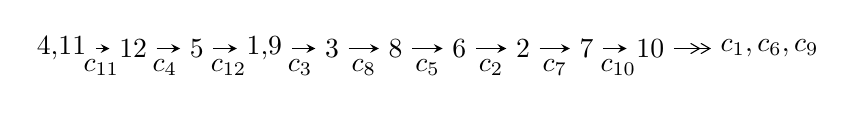
\begin{tikzpicture}[x=23pt, y=7pt]
	% node
	\node (A0) at (-1/8, 0) {4,11};
	\node (A1) at (1, 0) {12};
	\node (A2) at (2, 0) {5};
	\node (A3) at (49/16, 0) {1,9};
	\node (A4) at (33/8, 0) {3};
	\node (A5) at (41/8, 0) {8};
	\node (A6) at (49/8, 0) {6};
	\node (A7) at (57/8, 0) {2};
	\node (A8) at (65/8, 0) {7};
	\node (A9) at (73/8, 0) {10};
	\node (C1) at (1/2, -1) {$c_{11}$};
	\node (C2) at (3/2, -1) {$c_{4}$};
	\node (C3) at (5/2, -1) {$c_{12}$};
	\node (C4) at (29/8, -1) {$c_{3}$};
	\node (C5) at (37/8, -1) {$c_{8}$};
	\node (C6) at (45/8, -1) {$c_{5}$};
	\node (C7) at (53/8, -1) {$c_{2}$};
	\node (C8) at (61/8, -1) {$c_{7}$};
	\node (C9) at (69/8, -1) {$c_{10}$};
	\node (A10) at (11, 0) {$c_{1},c_{6},c_{9}$};

	% edge
	\draw[->,>=stealth]	
	(A0) edge (A1) (A1) edge (A2) (A2) edge (A3) (A3) edge (A4) (A4) edge (A5) (A5) edge (A6) (A6) edge (A7) (A7) edge (A8) (A8) edge (A9) ;
	\draw[->>,>={angle 60}]	
	(A9) edge (A10);
\end{tikzpicture} \\ 

\end{tabular} \\

\footnotetext{
The image of knot diagram is generated by the software ``\textbf{Draw programme}" developed by Andrew Bartholomew(\url{http://www.layer8.co.uk/maths/draw/index.htm\#Running-draw}), where we modified some parts for our purpose(\url{https://github.com/CATsTAILs/LinksPainter}).
}\phantom \\ \newline 
\centering \textbf{Ideals for irreducible components\footnotemark of $X_{\text{par}}$} 
 
\begin{align*}
I^u_{1}&=\langle 
-1.49961\times10^{89} u^{57}-4.30275\times10^{89} u^{56}+\cdots+1.84762\times10^{90} b-3.84519\times10^{90},\\
\phantom{I^u_{1}}&\phantom{= \langle  }9.24565\times10^{90} u^{57}+2.45942\times10^{91} u^{56}+\cdots+2.03238\times10^{91} a-1.65302\times10^{91},\;u^{58}+4 u^{57}+\cdots+32 u+11\rangle \\
I^u_{2}&=\langle 
2 u^{17}+u^{16}+\cdots+b-1,\\
\phantom{I^u_{2}}&\phantom{= \langle  }u^{16}-11 u^{14}+50 u^{12}- u^{11}-121 u^{10}+5 u^9+168 u^8-7 u^7-135 u^6- u^5+62 u^4+8 u^3-17 u^2+a-5 u+2,\\
\phantom{I^u_{2}}&\phantom{= \langle  }u^{18}- u^{17}+\cdots+2 u+1\rangle \\
\\
\end{align*}
\raggedright * 2 irreducible components of $\dim_{\mathbb{C}}=0$, with total 76 representations.\\
\footnotetext{All coefficients of polynomials are rational numbers. But the coefficients are sometimes approximated in decimal forms when there is not enough margin.}
\newpage
\renewcommand{\arraystretch}{1}
\centering \section*{I. $I^u_{1}= \langle -1.50\times10^{89} u^{57}-4.30\times10^{89} u^{56}+\cdots+1.85\times10^{90} b-3.85\times10^{90},\;9.25\times10^{90} u^{57}+2.46\times10^{91} u^{56}+\cdots+2.03\times10^{91} a-1.65\times10^{91},\;u^{58}+4 u^{57}+\cdots+32 u+11 \rangle$}
\flushleft \textbf{(i) Arc colorings}\\
\begin{tabular}{m{7pt} m{180pt} m{7pt} m{180pt} }
\flushright $a_{4}=$&$\begin{pmatrix}0\\u\end{pmatrix}$ \\
\flushright $a_{11}=$&$\begin{pmatrix}1\\0\end{pmatrix}$ \\
\flushright $a_{12}=$&$\begin{pmatrix}1\\- u^2\end{pmatrix}$ \\
\flushright $a_{5}=$&$\begin{pmatrix}u\\- u^3+u\end{pmatrix}$ \\
\flushright $a_{1}=$&$\begin{pmatrix}- u^2+1\\u^4-2 u^2\end{pmatrix}$ \\
\flushright $a_{9}=$&$\begin{pmatrix}-0.454916 u^{57}-1.21012 u^{56}+\cdots-16.5801 u+0.813340\\0.0811641 u^{57}+0.232880 u^{56}+\cdots-0.624802 u+2.08115\end{pmatrix}$ \\
\flushright $a_{3}=$&$\begin{pmatrix}-0.823019 u^{57}-2.12734 u^{56}+\cdots+7.49958 u-5.41326\\0.711078 u^{57}+1.92531 u^{56}+\cdots+19.8006 u+6.32004\end{pmatrix}$ \\
\flushright $a_{8}=$&$\begin{pmatrix}-0.536080 u^{57}-1.44300 u^{56}+\cdots-15.9553 u-1.26781\\0.0811641 u^{57}+0.232880 u^{56}+\cdots-0.624802 u+2.08115\end{pmatrix}$ \\
\flushright $a_{6}=$&$\begin{pmatrix}1.05675 u^{57}+2.85391 u^{56}+\cdots+27.8234 u+9.33471\\-0.544200 u^{57}-1.45256 u^{56}+\cdots-6.12029 u-4.46684\end{pmatrix}$ \\
\flushright $a_{2}=$&$\begin{pmatrix}-0.132988 u^{57}-0.334327 u^{56}+\cdots+12.2892 u-3.37486\\-0.0459035 u^{57}-0.0804690 u^{56}+\cdots+3.58707 u-1.18299\end{pmatrix}$ \\
\flushright $a_{7}=$&$\begin{pmatrix}-1.48462 u^{57}-3.93193 u^{56}+\cdots-27.9977 u-11.9930\\0.599967 u^{57}+1.56987 u^{56}+\cdots+8.28968 u+4.81357\end{pmatrix}$ \\
\flushright $a_{10}=$&$\begin{pmatrix}-1.04371 u^{57}-2.79063 u^{56}+\cdots-20.8363 u-7.03854\\0.545357 u^{57}+1.43212 u^{56}+\cdots+8.80444 u+4.70711\end{pmatrix}$\\&\end{tabular}
\flushleft \textbf{(ii) Obstruction class $= -1$}\\~\\
\flushleft \textbf{(iii) Cusp Shapes $= -2.03502 u^{57}-5.38837 u^{56}+\cdots-45.6934 u-9.66794$}\\~\\
\newpage\renewcommand{\arraystretch}{1}
\flushleft \textbf{(iv) u-Polynomials at the component}\newline \\
\begin{tabular}{m{50pt}|m{274pt}}
Crossings & \hspace{64pt}u-Polynomials at each crossing \\
\hline $$\begin{aligned}c_{1}\end{aligned}$$&$\begin{aligned}
&u^{58}+62 u^{57}+\cdots+142553 u+3481
\end{aligned}$\\
\hline $$\begin{aligned}c_{2},c_{7}\end{aligned}$$&$\begin{aligned}
&u^{58}-31 u^{56}+\cdots+3 u+59
\end{aligned}$\\
\hline $$\begin{aligned}c_{3},c_{9}\end{aligned}$$&$\begin{aligned}
&u^{58}- u^{57}+\cdots-2798 u+691
\end{aligned}$\\
\hline $$\begin{aligned}c_{4},c_{11},c_{12}\end{aligned}$$&$\begin{aligned}
&u^{58}-4 u^{57}+\cdots-32 u+11
\end{aligned}$\\
\hline $$\begin{aligned}c_{5}\end{aligned}$$&$\begin{aligned}
&u^{58}+12 u^{57}+\cdots+40669 u+11059
\end{aligned}$\\
\hline $$\begin{aligned}c_{6},c_{10}\end{aligned}$$&$\begin{aligned}
&u^{58}+2 u^{57}+\cdots-22 u+7
\end{aligned}$\\
\hline $$\begin{aligned}c_{8}\end{aligned}$$&$\begin{aligned}
&u^{58}-2 u^{57}+\cdots-471 u+43
\end{aligned}$\\
\hline
\end{tabular}\\~\\
\newpage\renewcommand{\arraystretch}{1}
\flushleft \textbf{(v) Riley Polynomials at the component}\newline \\
\begin{tabular}{m{50pt}|m{274pt}}
Crossings & \hspace{64pt}Riley Polynomials at each crossing \\
\hline $$\begin{aligned}c_{1}\end{aligned}$$&$\begin{aligned}
&y^{58}-114 y^{57}+\cdots+2999991563 y+12117361
\end{aligned}$\\
\hline $$\begin{aligned}c_{2},c_{7}\end{aligned}$$&$\begin{aligned}
&y^{58}-62 y^{57}+\cdots-142553 y+3481
\end{aligned}$\\
\hline $$\begin{aligned}c_{3},c_{9}\end{aligned}$$&$\begin{aligned}
&y^{58}+29 y^{57}+\cdots+3857388 y+477481
\end{aligned}$\\
\hline $$\begin{aligned}c_{4},c_{11},c_{12}\end{aligned}$$&$\begin{aligned}
&y^{58}-58 y^{57}+\cdots+8238 y+121
\end{aligned}$\\
\hline $$\begin{aligned}c_{5}\end{aligned}$$&$\begin{aligned}
&y^{58}+24 y^{57}+\cdots-2110306137 y+122301481
\end{aligned}$\\
\hline $$\begin{aligned}c_{6},c_{10}\end{aligned}$$&$\begin{aligned}
&y^{58}+20 y^{57}+\cdots+538 y+49
\end{aligned}$\\
\hline $$\begin{aligned}c_{8}\end{aligned}$$&$\begin{aligned}
&y^{58}-34 y^{57}+\cdots+76235 y+1849
\end{aligned}$\\
\hline
\end{tabular}\\~\\
\newpage\flushleft \textbf{(vi) Complex Volumes and Cusp Shapes}
$$\begin{array}{c|c|c}  
\text{Solutions to }I^u_{1}& \I (\text{vol} + \sqrt{-1}CS) & \text{Cusp shape}\\
 \hline 
\begin{aligned}
u &= -0.961036 + 0.344710 I \\
a &= \phantom{-}0.410562 - 0.361563 I \\
b &= \phantom{-}0.0577451 + 0.0746282 I\end{aligned}
 & \phantom{-}1.63603 - 1.28858 I & \phantom{-}3.68914 - 2.65059 I \\ \hline\begin{aligned}
u &= -0.961036 - 0.344710 I \\
a &= \phantom{-}0.410562 + 0.361563 I \\
b &= \phantom{-}0.0577451 - 0.0746282 I\end{aligned}
 & \phantom{-}1.63603 + 1.28858 I & \phantom{-}3.68914 + 2.65059 I \\ \hline\begin{aligned}
u &= -0.300610 + 0.983201 I \\
a &= -0.664168 + 0.542961 I \\
b &= -1.154320 + 0.289838 I\end{aligned}
 & \phantom{-}2.11065 - 4.12734 I & \phantom{-0.000000 -}0. + 10.48560 I \\ \hline\begin{aligned}
u &= -0.300610 - 0.983201 I \\
a &= -0.664168 - 0.542961 I \\
b &= -1.154320 - 0.289838 I\end{aligned}
 & \phantom{-}2.11065 + 4.12734 I & \phantom{-0.000000 } 0. - 10.48560 I \\ \hline\begin{aligned}
u &= \phantom{-}0.177176 + 1.016420 I \\
a &= \phantom{-}0.995049 + 0.839431 I \\
b &= \phantom{-}1.006590 + 0.559897 I\end{aligned}
 & -5.40198 + 2.14911 I & \phantom{-0.000000 } 0 \\ \hline\begin{aligned}
u &= \phantom{-}0.177176 - 1.016420 I \\
a &= \phantom{-}0.995049 - 0.839431 I \\
b &= \phantom{-}1.006590 - 0.559897 I\end{aligned}
 & -5.40198 - 2.14911 I & \phantom{-0.000000 } 0 \\ \hline\begin{aligned}
u &= \phantom{-}1.022550 + 0.300737 I \\
a &= \phantom{-}1.392440 - 0.121333 I \\
b &= -0.681814 - 0.288239 I\end{aligned}
 & -4.73896 - 0.44542 I & \phantom{-0.000000 } 0 \\ \hline\begin{aligned}
u &= \phantom{-}1.022550 - 0.300737 I \\
a &= \phantom{-}1.392440 + 0.121333 I \\
b &= -0.681814 + 0.288239 I\end{aligned}
 & -4.73896 + 0.44542 I & \phantom{-0.000000 } 0 \\ \hline\begin{aligned}
u &= \phantom{-}0.457539 + 1.028850 I \\
a &= -0.639770 - 1.028050 I \\
b &= -1.149000 - 0.599343 I\end{aligned}
 & -4.99783 + 9.61291 I & \phantom{-0.000000 } 0 \\ \hline\begin{aligned}
u &= \phantom{-}0.457539 - 1.028850 I \\
a &= -0.639770 + 1.028050 I \\
b &= -1.149000 + 0.599343 I\end{aligned}
 & -4.99783 - 9.61291 I & \phantom{-0.000000 } 0\\
 \hline 
 \end{array}$$\newpage$$\begin{array}{c|c|c}  
\text{Solutions to }I^u_{1}& \I (\text{vol} + \sqrt{-1}CS) & \text{Cusp shape}\\
 \hline 
\begin{aligned}
u &= -0.508367 + 0.560466 I \\
a &= \phantom{-}0.702577 - 1.074160 I \\
b &= \phantom{-}0.816859 - 0.437304 I\end{aligned}
 & \phantom{-}0.87869 - 1.96952 I & -2.93815 + 3.59463 I \\ \hline\begin{aligned}
u &= -0.508367 - 0.560466 I \\
a &= \phantom{-}0.702577 + 1.074160 I \\
b &= \phantom{-}0.816859 + 0.437304 I\end{aligned}
 & \phantom{-}0.87869 + 1.96952 I & -2.93815 - 3.59463 I \\ \hline\begin{aligned}
u &= -1.243480 + 0.160915 I \\
a &= -0.12542 + 1.47361 I \\
b &= -1.005060 + 0.654457 I\end{aligned}
 & \phantom{-}8.10144 - 2.64219 I & \phantom{-0.000000 } 0 \\ \hline\begin{aligned}
u &= -1.243480 - 0.160915 I \\
a &= -0.12542 - 1.47361 I \\
b &= -1.005060 - 0.654457 I\end{aligned}
 & \phantom{-}8.10144 + 2.64219 I & \phantom{-0.000000 } 0 \\ \hline\begin{aligned}
u &= \phantom{-}1.250380 + 0.115527 I \\
a &= -0.024680 + 0.709566 I \\
b &= \phantom{-}0.162747 + 1.279110 I\end{aligned}
 & \phantom{-}2.43342 + 2.95295 I & \phantom{-0.000000 } 0 \\ \hline\begin{aligned}
u &= \phantom{-}1.250380 - 0.115527 I \\
a &= -0.024680 - 0.709566 I \\
b &= \phantom{-}0.162747 - 1.279110 I\end{aligned}
 & \phantom{-}2.43342 - 2.95295 I & \phantom{-0.000000 } 0 \\ \hline\begin{aligned}
u &= \phantom{-}0.918632 + 0.898388 I \\
a &= -0.630878 - 0.202092 I \\
b &= -0.981209 + 0.316327 I\end{aligned}
 & -3.71484 - 3.13825 I & \phantom{-0.000000 } 0 \\ \hline\begin{aligned}
u &= \phantom{-}0.918632 - 0.898388 I \\
a &= -0.630878 + 0.202092 I \\
b &= -0.981209 - 0.316327 I\end{aligned}
 & -3.71484 + 3.13825 I & \phantom{-0.000000 } 0 \\ \hline\begin{aligned}
u &= -1.276100 + 0.238628 I \\
a &= \phantom{-}0.149526 + 0.895072 I \\
b &= \phantom{-}0.670232 + 1.202320 I\end{aligned}
 & -2.49632 - 0.10646 I & \phantom{-0.000000 } 0 \\ \hline\begin{aligned}
u &= -1.276100 - 0.238628 I \\
a &= \phantom{-}0.149526 - 0.895072 I \\
b &= \phantom{-}0.670232 - 1.202320 I\end{aligned}
 & -2.49632 + 0.10646 I & \phantom{-0.000000 } 0\\
 \hline 
 \end{array}$$\newpage$$\begin{array}{c|c|c}  
\text{Solutions to }I^u_{1}& \I (\text{vol} + \sqrt{-1}CS) & \text{Cusp shape}\\
 \hline 
\begin{aligned}
u &= \phantom{-}0.214091 + 0.659200 I \\
a &= \phantom{-}0.42003 + 1.64314 I \\
b &= -0.474121 + 0.960246 I\end{aligned}
 & -7.21101 + 3.94882 I & -5.14255 - 3.51346 I \\ \hline\begin{aligned}
u &= \phantom{-}0.214091 - 0.659200 I \\
a &= \phantom{-}0.42003 - 1.64314 I \\
b &= -0.474121 - 0.960246 I\end{aligned}
 & -7.21101 - 3.94882 I & -5.14255 + 3.51346 I \\ \hline\begin{aligned}
u &= -1.340150 + 0.006307 I \\
a &= -0.671961 - 0.615224 I \\
b &= \phantom{-}1.44910 - 0.06502 I\end{aligned}
 & \phantom{-}6.41008 + 2.01791 I & \phantom{-0.000000 } 0 \\ \hline\begin{aligned}
u &= -1.340150 - 0.006307 I \\
a &= -0.671961 + 0.615224 I \\
b &= \phantom{-}1.44910 + 0.06502 I\end{aligned}
 & \phantom{-}6.41008 - 2.01791 I & \phantom{-0.000000 } 0 \\ \hline\begin{aligned}
u &= \phantom{-}1.208760 + 0.634237 I \\
a &= \phantom{-}0.615633 + 0.389195 I \\
b &= \phantom{-}0.868802 - 0.223405 I\end{aligned}
 & -2.30604 + 3.66617 I & \phantom{-0.000000 } 0 \\ \hline\begin{aligned}
u &= \phantom{-}1.208760 - 0.634237 I \\
a &= \phantom{-}0.615633 - 0.389195 I \\
b &= \phantom{-}0.868802 + 0.223405 I\end{aligned}
 & -2.30604 - 3.66617 I & \phantom{-0.000000 } 0 \\ \hline\begin{aligned}
u &= \phantom{-}1.361830 + 0.160284 I \\
a &= -0.384112 + 0.899780 I \\
b &= \phantom{-}1.46541 + 0.58759 I\end{aligned}
 & \phantom{-}6.81065 + 3.86139 I & \phantom{-0.000000 } 0 \\ \hline\begin{aligned}
u &= \phantom{-}1.361830 - 0.160284 I \\
a &= -0.384112 - 0.899780 I \\
b &= \phantom{-}1.46541 - 0.58759 I\end{aligned}
 & \phantom{-}6.81065 - 3.86139 I & \phantom{-0.000000 } 0 \\ \hline\begin{aligned}
u &= \phantom{-}1.357900 + 0.198010 I \\
a &= -1.41096 - 0.24260 I \\
b &= \phantom{-}0.980223 + 0.173254 I\end{aligned}
 & -2.00761 + 5.36474 I & \phantom{-0.000000 } 0 \\ \hline\begin{aligned}
u &= \phantom{-}1.357900 - 0.198010 I \\
a &= -1.41096 + 0.24260 I \\
b &= \phantom{-}0.980223 - 0.173254 I\end{aligned}
 & -2.00761 - 5.36474 I & \phantom{-0.000000 } 0\\
 \hline 
 \end{array}$$\newpage$$\begin{array}{c|c|c}  
\text{Solutions to }I^u_{1}& \I (\text{vol} + \sqrt{-1}CS) & \text{Cusp shape}\\
 \hline 
\begin{aligned}
u &= -0.351158 + 0.438829 I \\
a &= -1.90822 + 1.84789 I \\
b &= -0.931746 - 0.128227 I\end{aligned}
 & \phantom{-}5.20133 + 0.56913 I & \phantom{-}3.17376 + 3.13957 I \\ \hline\begin{aligned}
u &= -0.351158 - 0.438829 I \\
a &= -1.90822 - 1.84789 I \\
b &= -0.931746 + 0.128227 I\end{aligned}
 & \phantom{-}5.20133 - 0.56913 I & \phantom{-}3.17376 - 3.13957 I \\ \hline\begin{aligned}
u &= -1.41665 + 0.25497 I \\
a &= -0.167580 - 0.716545 I \\
b &= -0.39722 - 1.42369 I\end{aligned}
 & -1.94189 - 7.25945 I & \phantom{-0.000000 } 0 \\ \hline\begin{aligned}
u &= -1.41665 - 0.25497 I \\
a &= -0.167580 + 0.716545 I \\
b &= -0.39722 + 1.42369 I\end{aligned}
 & -1.94189 + 7.25945 I & \phantom{-0.000000 } 0 \\ \hline\begin{aligned}
u &= -1.38880 + 0.42731 I \\
a &= \phantom{-}0.271840 + 0.657054 I \\
b &= -1.238430 + 0.075451 I\end{aligned}
 & \phantom{-}5.55129 - 1.69307 I & \phantom{-0.000000 } 0 \\ \hline\begin{aligned}
u &= -1.38880 - 0.42731 I \\
a &= \phantom{-}0.271840 - 0.657054 I \\
b &= -1.238430 - 0.075451 I\end{aligned}
 & \phantom{-}5.55129 + 1.69307 I & \phantom{-0.000000 } 0 \\ \hline\begin{aligned}
u &= -0.020913 + 0.538103 I \\
a &= -1.45595 - 2.11846 I \\
b &= \phantom{-}0.699320 - 0.714521 I\end{aligned}
 & -6.48919 - 2.77189 I & -4.31702 + 3.80378 I \\ \hline\begin{aligned}
u &= -0.020913 - 0.538103 I \\
a &= -1.45595 + 2.11846 I \\
b &= \phantom{-}0.699320 + 0.714521 I\end{aligned}
 & -6.48919 + 2.77189 I & -4.31702 - 3.80378 I \\ \hline\begin{aligned}
u &= -1.40623 + 0.43425 I \\
a &= -0.151715 - 1.142070 I \\
b &= \phantom{-}1.25232 - 0.77633 I\end{aligned}
 & -0.39560 - 7.30241 I & \phantom{-0.000000 } 0 \\ \hline\begin{aligned}
u &= -1.40623 - 0.43425 I \\
a &= -0.151715 + 1.142070 I \\
b &= \phantom{-}1.25232 + 0.77633 I\end{aligned}
 & -0.39560 + 7.30241 I & \phantom{-0.000000 } 0\\
 \hline 
 \end{array}$$\newpage$$\begin{array}{c|c|c}  
\text{Solutions to }I^u_{1}& \I (\text{vol} + \sqrt{-1}CS) & \text{Cusp shape}\\
 \hline 
\begin{aligned}
u &= \phantom{-}1.46204 + 0.36462 I \\
a &= \phantom{-}0.326405 - 0.912619 I \\
b &= -1.44645 - 0.46355 I\end{aligned}
 & \phantom{-}7.77629 + 8.86284 I & \phantom{-0.000000 } 0 \\ \hline\begin{aligned}
u &= \phantom{-}1.46204 - 0.36462 I \\
a &= \phantom{-}0.326405 + 0.912619 I \\
b &= -1.44645 + 0.46355 I\end{aligned}
 & \phantom{-}7.77629 - 8.86284 I & \phantom{-0.000000 } 0 \\ \hline\begin{aligned}
u &= \phantom{-}0.443286 + 0.212059 I \\
a &= -0.662346 + 0.537430 I \\
b &= \phantom{-}0.716948 + 0.729738 I\end{aligned}
 & \phantom{-}0.67091 + 2.53345 I & -6.84359 - 5.09477 I \\ \hline\begin{aligned}
u &= \phantom{-}0.443286 - 0.212059 I \\
a &= -0.662346 - 0.537430 I \\
b &= \phantom{-}0.716948 - 0.729738 I\end{aligned}
 & \phantom{-}0.67091 - 2.53345 I & -6.84359 + 5.09477 I \\ \hline\begin{aligned}
u &= \phantom{-}0.105029 + 0.468274 I \\
a &= \phantom{-}0.858036 - 0.852783 I \\
b &= -0.148908 - 0.554790 I\end{aligned}
 & -0.879280 - 0.837953 I & -6.06157 + 3.85318 I \\ \hline\begin{aligned}
u &= \phantom{-}0.105029 - 0.468274 I \\
a &= \phantom{-}0.858036 + 0.852783 I \\
b &= -0.148908 + 0.554790 I\end{aligned}
 & -0.879280 + 0.837953 I & -6.06157 - 3.85318 I \\ \hline\begin{aligned}
u &= \phantom{-}1.52144 + 0.16063 I \\
a &= \phantom{-}0.147683 - 1.054080 I \\
b &= -0.988171 - 0.419538 I\end{aligned}
 & \phantom{-}11.65080 + 1.76628 I & \phantom{-0.000000 } 0 \\ \hline\begin{aligned}
u &= \phantom{-}1.52144 - 0.16063 I \\
a &= \phantom{-}0.147683 + 1.054080 I \\
b &= -0.988171 + 0.419538 I\end{aligned}
 & \phantom{-}11.65080 - 1.76628 I & \phantom{-0.000000 } 0 \\ \hline\begin{aligned}
u &= -1.55510 + 0.06787 I \\
a &= -0.415660 - 0.379485 I \\
b &= \phantom{-}1.24881 - 0.70054 I\end{aligned}
 & \phantom{-}7.53900 - 3.50491 I & \phantom{-0.000000 } 0 \\ \hline\begin{aligned}
u &= -1.55510 - 0.06787 I \\
a &= -0.415660 + 0.379485 I \\
b &= \phantom{-}1.24881 + 0.70054 I\end{aligned}
 & \phantom{-}7.53900 + 3.50491 I & \phantom{-0.000000 } 0\\
 \hline 
 \end{array}$$\newpage$$\begin{array}{c|c|c}  
\text{Solutions to }I^u_{1}& \I (\text{vol} + \sqrt{-1}CS) & \text{Cusp shape}\\
 \hline 
\begin{aligned}
u &= \phantom{-}1.55296 + 0.10743 I \\
a &= -0.265564 + 0.772783 I \\
b &= \phantom{-}1.29007 + 0.93480 I\end{aligned}
 & \phantom{-}7.76727 + 4.14815 I & \phantom{-0.000000 } 0 \\ \hline\begin{aligned}
u &= \phantom{-}1.55296 - 0.10743 I \\
a &= -0.265564 - 0.772783 I \\
b &= \phantom{-}1.29007 - 0.93480 I\end{aligned}
 & \phantom{-}7.76727 - 4.14815 I & \phantom{-0.000000 } 0 \\ \hline\begin{aligned}
u &= -1.54876 + 0.39196 I \\
a &= \phantom{-}0.309319 + 1.063530 I \\
b &= -1.38659 + 0.73109 I\end{aligned}
 & \phantom{-}1.4411 - 14.7651 I & \phantom{-0.000000 } 0 \\ \hline\begin{aligned}
u &= -1.54876 - 0.39196 I \\
a &= \phantom{-}0.309319 - 1.063530 I \\
b &= -1.38659 - 0.73109 I\end{aligned}
 & \phantom{-}1.4411 + 14.7651 I & \phantom{-0.000000 } 0 \\ \hline\begin{aligned}
u &= -1.69455 + 0.13644 I \\
a &= \phantom{-}0.354754 + 0.421724 I \\
b &= -0.995880 + 0.147977 I\end{aligned}
 & \phantom{-}5.71581 - 0.60212 I & \phantom{-0.000000 } 0 \\ \hline\begin{aligned}
u &= -1.69455 - 0.13644 I \\
a &= \phantom{-}0.354754 - 0.421724 I \\
b &= -0.995880 - 0.147977 I\end{aligned}
 & \phantom{-}5.71581 + 0.60212 I & \phantom{-0.000000 } 0 \\ \hline\begin{aligned}
u &= -0.041702 + 0.155977 I \\
a &= \phantom{-}4.67058 - 1.41112 I \\
b &= \phantom{-}1.293750 - 0.398711 I\end{aligned}
 & \phantom{-}2.00910 - 2.36209 I & \phantom{-}6.75260 - 1.70759 I \\ \hline\begin{aligned}
u &= -0.041702 - 0.155977 I \\
a &= \phantom{-}4.67058 + 1.41112 I \\
b &= \phantom{-}1.293750 + 0.398711 I\end{aligned}
 & \phantom{-}2.00910 + 2.36209 I & \phantom{-}6.75260 + 1.70759 I\\
 \hline 
 \end{array}$$\newpage\newpage\renewcommand{\arraystretch}{1}
\centering \section*{II. $I^u_{2}= \langle 2 u^{17}+u^{16}+\cdots+b-1,\;u^{16}-11 u^{14}+\cdots+a+2,\;u^{18}- u^{17}+\cdots+2 u+1 \rangle$}
\flushleft \textbf{(i) Arc colorings}\\
\begin{tabular}{m{7pt} m{180pt} m{7pt} m{180pt} }
\flushright $a_{4}=$&$\begin{pmatrix}0\\u\end{pmatrix}$ \\
\flushright $a_{11}=$&$\begin{pmatrix}1\\0\end{pmatrix}$ \\
\flushright $a_{12}=$&$\begin{pmatrix}1\\- u^2\end{pmatrix}$ \\
\flushright $a_{5}=$&$\begin{pmatrix}u\\- u^3+u\end{pmatrix}$ \\
\flushright $a_{1}=$&$\begin{pmatrix}- u^2+1\\u^4-2 u^2\end{pmatrix}$ \\
\flushright $a_{9}=$&$\begin{pmatrix}- u^{16}+11 u^{14}+\cdots+5 u-2\\-2 u^{17}- u^{16}+\cdots+5 u+1\end{pmatrix}$ \\
\flushright $a_{3}=$&$\begin{pmatrix}u^{17}-2 u^{16}+\cdots+19 u+4\\2 u^{17}-21 u^{15}+\cdots-10 u^2+2 u\end{pmatrix}$ \\
\flushright $a_{8}=$&$\begin{pmatrix}2 u^{17}-20 u^{15}+\cdots+2 u^2-3\\-2 u^{17}- u^{16}+\cdots+5 u+1\end{pmatrix}$ \\
\flushright $a_{6}=$&$\begin{pmatrix}3 u^{17}-31 u^{15}+\cdots-7 u^2+7 u\\- u^{17}+10 u^{15}+\cdots+5 u+1\end{pmatrix}$ \\
\flushright $a_{2}=$&$\begin{pmatrix}2 u^{17}-2 u^{16}+\cdots+18 u+1\\2 u^{17}-21 u^{15}+\cdots+2 u-1\end{pmatrix}$ \\
\flushright $a_{7}=$&$\begin{pmatrix}- u^{17}+u^{16}+\cdots-12 u-1\\u^{16}-10 u^{14}+\cdots-5 u-1\end{pmatrix}$ \\
\flushright $a_{10}=$&$\begin{pmatrix}u^{16}- u^{15}+\cdots- u+4\\u^{16}-10 u^{14}+\cdots- u+1\end{pmatrix}$\\&\end{tabular}
\flushleft \textbf{(ii) Obstruction class $= 1$}\\~\\
\flushleft \textbf{(iii) Cusp Shapes $= -3 u^{17}-7 u^{16}+30 u^{15}+69 u^{14}-127 u^{13}-279 u^{12}+295 u^{11}+593 u^{10}-398 u^9-710 u^8+286 u^7+484 u^6-61 u^5-186 u^4-42 u^3+33 u^2+27 u+8$}\\~\\
\newpage\renewcommand{\arraystretch}{1}
\flushleft \textbf{(iv) u-Polynomials at the component}\newline \\
\begin{tabular}{m{50pt}|m{274pt}}
Crossings & \hspace{64pt}u-Polynomials at each crossing \\
\hline $$\begin{aligned}c_{1}\end{aligned}$$&$\begin{aligned}
&u^{18}-19 u^{17}+\cdots+7 u+1
\end{aligned}$\\
\hline $$\begin{aligned}c_{2}\end{aligned}$$&$\begin{aligned}
&u^{18}+u^{17}+\cdots+u+1
\end{aligned}$\\
\hline $$\begin{aligned}c_{3}\end{aligned}$$&$\begin{aligned}
&u^{18}+6 u^{16}+\cdots+12 u^2+1
\end{aligned}$\\
\hline $$\begin{aligned}c_{4}\end{aligned}$$&$\begin{aligned}
&u^{18}+u^{17}+\cdots-2 u+1
\end{aligned}$\\
\hline $$\begin{aligned}c_{5}\end{aligned}$$&$\begin{aligned}
&u^{18}- u^{17}+\cdots+637 u+169
\end{aligned}$\\
\hline $$\begin{aligned}c_{6}\end{aligned}$$&$\begin{aligned}
&u^{18}+u^{17}+\cdots+9 u^2+1
\end{aligned}$\\
\hline $$\begin{aligned}c_{7}\end{aligned}$$&$\begin{aligned}
&u^{18}- u^{17}+\cdots- u+1
\end{aligned}$\\
\hline $$\begin{aligned}c_{8}\end{aligned}$$&$\begin{aligned}
&u^{18}+3 u^{17}+\cdots+3 u+1
\end{aligned}$\\
\hline $$\begin{aligned}c_{9}\end{aligned}$$&$\begin{aligned}
&u^{18}+6 u^{16}+\cdots+12 u^2+1
\end{aligned}$\\
\hline $$\begin{aligned}c_{10}\end{aligned}$$&$\begin{aligned}
&u^{18}- u^{17}+\cdots+9 u^2+1
\end{aligned}$\\
\hline $$\begin{aligned}c_{11},c_{12}\end{aligned}$$&$\begin{aligned}
&u^{18}- u^{17}+\cdots+2 u+1
\end{aligned}$\\
\hline
\end{tabular}\\~\\
\newpage\renewcommand{\arraystretch}{1}
\flushleft \textbf{(v) Riley Polynomials at the component}\newline \\
\begin{tabular}{m{50pt}|m{274pt}}
Crossings & \hspace{64pt}Riley Polynomials at each crossing \\
\hline $$\begin{aligned}c_{1}\end{aligned}$$&$\begin{aligned}
&y^{18}-23 y^{17}+\cdots-113 y+1
\end{aligned}$\\
\hline $$\begin{aligned}c_{2},c_{7}\end{aligned}$$&$\begin{aligned}
&y^{18}-19 y^{17}+\cdots+7 y+1
\end{aligned}$\\
\hline $$\begin{aligned}c_{3},c_{9}\end{aligned}$$&$\begin{aligned}
&y^{18}+12 y^{17}+\cdots+24 y+1
\end{aligned}$\\
\hline $$\begin{aligned}c_{4},c_{11},c_{12}\end{aligned}$$&$\begin{aligned}
&y^{18}-23 y^{17}+\cdots+10 y+1
\end{aligned}$\\
\hline $$\begin{aligned}c_{5}\end{aligned}$$&$\begin{aligned}
&y^{18}- y^{17}+\cdots+80275 y+28561
\end{aligned}$\\
\hline $$\begin{aligned}c_{6},c_{10}\end{aligned}$$&$\begin{aligned}
&y^{18}+15 y^{17}+\cdots+18 y+1
\end{aligned}$\\
\hline $$\begin{aligned}c_{8}\end{aligned}$$&$\begin{aligned}
&y^{18}-11 y^{17}+\cdots+3 y+1
\end{aligned}$\\
\hline
\end{tabular}\\~\\
\newpage\flushleft \textbf{(vi) Complex Volumes and Cusp Shapes}
$$\begin{array}{c|c|c}  
\text{Solutions to }I^u_{2}& \I (\text{vol} + \sqrt{-1}CS) & \text{Cusp shape}\\
 \hline 
\begin{aligned}
u &= -0.887779 + 0.112048 I \\
a &= \phantom{-}0.089265 - 0.331367 I \\
b &= \phantom{-}0.461534 - 0.749043 I\end{aligned}
 & \phantom{-}1.39736 - 2.22617 I & \phantom{-}1.56231 + 2.33825 I \\ \hline\begin{aligned}
u &= -0.887779 - 0.112048 I \\
a &= \phantom{-}0.089265 + 0.331367 I \\
b &= \phantom{-}0.461534 + 0.749043 I\end{aligned}
 & \phantom{-}1.39736 + 2.22617 I & \phantom{-}1.56231 - 2.33825 I \\ \hline\begin{aligned}
u &= \phantom{-}0.758736 + 0.433252 I \\
a &= -0.977741 + 0.684412 I \\
b &= \phantom{-}0.369099 - 0.429483 I\end{aligned}
 & -5.13432 - 1.67601 I & -1.62747 + 2.23910 I \\ \hline\begin{aligned}
u &= \phantom{-}0.758736 - 0.433252 I \\
a &= -0.977741 - 0.684412 I \\
b &= \phantom{-}0.369099 + 0.429483 I\end{aligned}
 & -5.13432 + 1.67601 I & -1.62747 - 2.23910 I \\ \hline\begin{aligned}
u &= \phantom{-}1.143310 + 0.336155 I \\
a &= \phantom{-}0.949765 + 0.051215 I \\
b &= \phantom{-}0.058602 + 0.523758 I\end{aligned}
 & -3.76019 + 4.59860 I & -1.93853 - 3.26173 I \\ \hline\begin{aligned}
u &= \phantom{-}1.143310 - 0.336155 I \\
a &= \phantom{-}0.949765 - 0.051215 I \\
b &= \phantom{-}0.058602 - 0.523758 I\end{aligned}
 & -3.76019 - 4.59860 I & -1.93853 + 3.26173 I \\ \hline\begin{aligned}
u &= -0.383102 + 0.444250 I \\
a &= \phantom{-}0.823217 - 0.923482 I \\
b &= \phantom{-}1.133460 - 0.522137 I\end{aligned}
 & \phantom{-}1.76189 - 2.88146 I & \phantom{-}1.41103 + 9.64361 I \\ \hline\begin{aligned}
u &= -0.383102 - 0.444250 I \\
a &= \phantom{-}0.823217 + 0.923482 I \\
b &= \phantom{-}1.133460 + 0.522137 I\end{aligned}
 & \phantom{-}1.76189 + 2.88146 I & \phantom{-}1.41103 - 9.64361 I \\ \hline\begin{aligned}
u &= -1.45384 + 0.15707 I \\
a &= \phantom{-}0.292000 + 1.088040 I \\
b &= -1.046950 + 0.117848 I\end{aligned}
 & \phantom{-}9.99566 - 0.53098 I & \phantom{-}4.50651 - 0.51925 I \\ \hline\begin{aligned}
u &= -1.45384 - 0.15707 I \\
a &= \phantom{-}0.292000 - 1.088040 I \\
b &= -1.046950 - 0.117848 I\end{aligned}
 & \phantom{-}9.99566 + 0.53098 I & \phantom{-}4.50651 + 0.51925 I\\
 \hline 
 \end{array}$$\newpage$$\begin{array}{c|c|c}  
\text{Solutions to }I^u_{2}& \I (\text{vol} + \sqrt{-1}CS) & \text{Cusp shape}\\
 \hline 
\begin{aligned}
u &= \phantom{-}1.48783 + 0.11385 I \\
a &= \phantom{-}0.078910 - 1.084200 I \\
b &= -1.091720 - 0.722143 I\end{aligned}
 & \phantom{-}10.62920 + 2.91434 I & \phantom{-}4.17629 - 3.27745 I \\ \hline\begin{aligned}
u &= \phantom{-}1.48783 - 0.11385 I \\
a &= \phantom{-}0.078910 + 1.084200 I \\
b &= -1.091720 + 0.722143 I\end{aligned}
 & \phantom{-}10.62920 - 2.91434 I & \phantom{-}4.17629 + 3.27745 I \\ \hline\begin{aligned}
u &= \phantom{-}1.54419 + 0.09001 I \\
a &= -0.288335 + 0.654660 I \\
b &= \phantom{-}1.44443 + 0.99383 I\end{aligned}
 & \phantom{-}8.50423 + 4.51006 I & \phantom{-}9.09047 - 7.39147 I \\ \hline\begin{aligned}
u &= \phantom{-}1.54419 - 0.09001 I \\
a &= -0.288335 - 0.654660 I \\
b &= \phantom{-}1.44443 - 0.99383 I\end{aligned}
 & \phantom{-}8.50423 - 4.51006 I & \phantom{-}9.09047 + 7.39147 I \\ \hline\begin{aligned}
u &= -1.64388 + 0.28012 I \\
a &= -0.301507 - 0.405678 I \\
b &= \phantom{-}1.183200 - 0.160247 I\end{aligned}
 & \phantom{-}6.07303 - 1.21729 I & \phantom{-}10.42303 + 3.11644 I \\ \hline\begin{aligned}
u &= -1.64388 - 0.28012 I \\
a &= -0.301507 + 0.405678 I \\
b &= \phantom{-}1.183200 + 0.160247 I\end{aligned}
 & \phantom{-}6.07303 + 1.21729 I & \phantom{-}10.42303 - 3.11644 I \\ \hline\begin{aligned}
u &= -0.065465 + 0.318414 I \\
a &= -4.66557 + 0.43662 I \\
b &= -1.011650 + 0.306442 I\end{aligned}
 & \phantom{-}5.07676 - 1.32129 I & \phantom{-}0.89638 + 6.13933 I \\ \hline\begin{aligned}
u &= -0.065465 - 0.318414 I \\
a &= -4.66557 - 0.43662 I \\
b &= -1.011650 - 0.306442 I\end{aligned}
 & \phantom{-}5.07676 + 1.32129 I & \phantom{-}0.89638 - 6.13933 I\\
 \hline 
 \end{array}$$\newpage
\newpage\renewcommand{\arraystretch}{1}
\centering \section*{ III. u-Polynomials}
\begin{tabular}{m{50pt}|m{274pt}}
Crossings & \hspace{64pt}u-Polynomials at each crossing \\
\hline $$\begin{aligned}c_{1}\end{aligned}$$&$\begin{aligned}
&(u^{18}-19 u^{17}+\cdots+7 u+1)(u^{58}+62 u^{57}+\cdots+142553 u+3481)
\end{aligned}$\\
\hline $$\begin{aligned}c_{2}\end{aligned}$$&$\begin{aligned}
&(u^{18}+u^{17}+\cdots+u+1)(u^{58}-31 u^{56}+\cdots+3 u+59)
\end{aligned}$\\
\hline $$\begin{aligned}c_{3}\end{aligned}$$&$\begin{aligned}
&(u^{18}+6 u^{16}+\cdots+12 u^2+1)(u^{58}- u^{57}+\cdots-2798 u+691)
\end{aligned}$\\
\hline $$\begin{aligned}c_{4}\end{aligned}$$&$\begin{aligned}
&(u^{18}+u^{17}+\cdots-2 u+1)(u^{58}-4 u^{57}+\cdots-32 u+11)
\end{aligned}$\\
\hline $$\begin{aligned}c_{5}\end{aligned}$$&$\begin{aligned}
&(u^{18}- u^{17}+\cdots+637 u+169)(u^{58}+12 u^{57}+\cdots+40669 u+11059)
\end{aligned}$\\
\hline $$\begin{aligned}c_{6}\end{aligned}$$&$\begin{aligned}
&(u^{18}+u^{17}+\cdots+9 u^2+1)(u^{58}+2 u^{57}+\cdots-22 u+7)
\end{aligned}$\\
\hline $$\begin{aligned}c_{7}\end{aligned}$$&$\begin{aligned}
&(u^{18}- u^{17}+\cdots- u+1)(u^{58}-31 u^{56}+\cdots+3 u+59)
\end{aligned}$\\
\hline $$\begin{aligned}c_{8}\end{aligned}$$&$\begin{aligned}
&(u^{18}+3 u^{17}+\cdots+3 u+1)(u^{58}-2 u^{57}+\cdots-471 u+43)
\end{aligned}$\\
\hline $$\begin{aligned}c_{9}\end{aligned}$$&$\begin{aligned}
&(u^{18}+6 u^{16}+\cdots+12 u^2+1)(u^{58}- u^{57}+\cdots-2798 u+691)
\end{aligned}$\\
\hline $$\begin{aligned}c_{10}\end{aligned}$$&$\begin{aligned}
&(u^{18}- u^{17}+\cdots+9 u^2+1)(u^{58}+2 u^{57}+\cdots-22 u+7)
\end{aligned}$\\
\hline $$\begin{aligned}c_{11},c_{12}\end{aligned}$$&$\begin{aligned}
&(u^{18}- u^{17}+\cdots+2 u+1)(u^{58}-4 u^{57}+\cdots-32 u+11)
\end{aligned}$\\
\hline
\end{tabular}\newpage\renewcommand{\arraystretch}{1}
\centering \section*{ IV. Riley Polynomials}
\begin{tabular}{m{50pt}|m{274pt}}
Crossings & \hspace{64pt}Riley Polynomials at each crossing \\
\hline $$\begin{aligned}c_{1}\end{aligned}$$&$\begin{aligned}
&(y^{18}-23 y^{17}+\cdots-113 y+1)\\
&\cdot(y^{58}-114 y^{57}+\cdots+2999991563 y+12117361)
\end{aligned}$\\
\hline $$\begin{aligned}c_{2},c_{7}\end{aligned}$$&$\begin{aligned}
&(y^{18}-19 y^{17}+\cdots+7 y+1)(y^{58}-62 y^{57}+\cdots-142553 y+3481)
\end{aligned}$\\
\hline $$\begin{aligned}c_{3},c_{9}\end{aligned}$$&$\begin{aligned}
&(y^{18}+12 y^{17}+\cdots+24 y+1)\\
&\cdot(y^{58}+29 y^{57}+\cdots+3857388 y+477481)
\end{aligned}$\\
\hline $$\begin{aligned}c_{4},c_{11},c_{12}\end{aligned}$$&$\begin{aligned}
&(y^{18}-23 y^{17}+\cdots+10 y+1)(y^{58}-58 y^{57}+\cdots+8238 y+121)
\end{aligned}$\\
\hline $$\begin{aligned}c_{5}\end{aligned}$$&$\begin{aligned}
&(y^{18}- y^{17}+\cdots+80275 y+28561)\\
&\cdot(y^{58}+24 y^{57}+\cdots-2110306137 y+122301481)
\end{aligned}$\\
\hline $$\begin{aligned}c_{6},c_{10}\end{aligned}$$&$\begin{aligned}
&(y^{18}+15 y^{17}+\cdots+18 y+1)(y^{58}+20 y^{57}+\cdots+538 y+49)
\end{aligned}$\\
\hline $$\begin{aligned}c_{8}\end{aligned}$$&$\begin{aligned}
&(y^{18}-11 y^{17}+\cdots+3 y+1)(y^{58}-34 y^{57}+\cdots+76235 y+1849)
\end{aligned}$\\
\hline
\end{tabular}
\vskip 2pc
\end{document}